\documentclass[mathserif]{intbeamer}
%\usepackage{etex}
\usepackage[utf8]{inputenc}
\usepackage[english]{babel}
%\usepackage{qrcode}
%\usepackage[space]{grffile}
\usepackage{subcaption}
\captionsetup[subfigure]{skip=-5pt} % global setting for subfigure
%\usepackage{aligned-overset}
\usepackage{trfsigns}

\usepackage{../paper/macros}
\usepackage{xcolor}

\makeatletter
\def\mathcolor#1#{\@mathcolor{#1}}
\def\@mathcolor#1#2#3{%
  \protect\leavevmode
  \begingroup
    \color#1{#2}#3%
  \endgroup
}
\makeatother


%% *** Tikz, PGF and AudioIcons ***
%\usepackage{tikz, audioicons}
%\usetikzlibrary{calc,%
%  decorations.pathreplacing,%
  % decorations.markings,%
  % calc,%
  % arrows,%
  % through,%
  % intersections,%
  % positioning}

%\definecolor{activecolor}{RGB}{255, 0, 0}
% \definecolor{loudspeakercircle}{RGB}{236, 236, 236}
% \definecolor{focuscircle}{RGB}{254, 204, 0}
% \definecolor{darkgreen}{rgb}{0,0.5,0}
% \definecolor{orange}{rgb}{1.0,0.5,0}
% \definecolor{mauve}{RGB}{224,176,255}
% \definecolor{teal}{RGB}{64,224,208}

% \makeatletter
% \tikzset{
%   dot diameter/.store in=\dot@diameter,
%   dot diameter=3pt,
%   dot spacing/.store in=\dot@spacing,
%   dot spacing=10pt,
%   dots/.style={
%     line width=\dot@diameter,
%     line cap=round,
%     dash pattern=on 0pt off \dot@spacing
%   }
% }
% \makeatother

%% *** Importing Stuff ***
%\usepackage{import}

%% *** Mathsymbols ***
%\usepackage{soundfield}
%\sfrenewsymbol{cylm}{\mu}

%\usepackage{nicefrac}
%\DeclareFontFamily{U}{wncy}{}
%\DeclareFontShape{U}{wncy}{m}{n}{<->wncyr10}{}
%\DeclareSymbolFont{mcy}{U}{wncy}{m}{n}
%\DeclareMathSymbol{\Sha}{\mathord}{mcy}{"58}

%% *** Additional Commands extending Beamer ***
%\newcommand{\itemplus}[1][+]{\item[\textcolor{darkgreen}{\textbf{#1}}]}
%\newcommand{\itemminus}[1][--]{\item[\textcolor{red}{\textbf{#1}}]}
%\newcommand{\itemattent}[1][!\,]{\item[\textcolor{orange}{\textbf{#1}}]}
%\newcommand{\itemcheck}{\itemplus[$\checkmark$]}
%\newcommand{\itemcross}{\itemminus[$\boldsymbol{\times}$]}

%\newenvironment{itemizeblock}[1]{ %
%  \begin{block}{#1} %
%    \begin{itemize} %
%    } %
%    { %
%    \end{itemize} %
%  \end{block} %
%} %

\setbeamercovered{invisible}

% ===== titlepage info =====
\title[Audibility Constant Phase Shifts]%
  {Detection of Constant Phase Shifts in\\Filters for Sound Field Synthesis}

\author[Schultz, Hahn, Spors]{%
    \underline{Frank Schultz},
    Nara Hahn,
    Sascha Spors
}

\date[2019-09-28]{%
  5th ICSA, Ilmenau, ORAL-5-3\\
}

\institute[]{Institute of Communications Engineering, University of Rostock}

% ===== remove total number of slides from pagenumber =====
\setbeamertemplate{page number in head/foot}[nototal]
\setbeamersize{text margin left=\logomargin}
\setbeamertemplate{blocks}[rounded]
\setbeamercolor{block title}{fg=rostock-uni, bg=white}

\begin{document}
\maketitle
%
%
%
\section{Introduction}
\begin{frame}{Sound Field Synthesis (SFS) with Linear / Planar Arrays}

\begin{columns}[T]
\column{0.33\textwidth}
2.5-dimensional SFS

\hspace{1cm}\includegraphics[width=0.5\textwidth]{graphics/LineArray_Slides}
\column{0.67\textwidth}
\only<1>{
%\includegraphics[width=1\textwidth]{graphics/Ideal3dB45deg}
ideal half-derivative filter for infinite linear array}
\only<2>{
%\includegraphics[width=.45\textwidth]{graphics/Coupling3dB}
%\includegraphics[width=.45\textwidth]{graphics/PhaseTypes}
}
\end{columns}
\vspace{0.5cm}
\begin{columns}[T]
\column{0.33\textwidth}
3-dimensional SFS

\includegraphics[width=1\textwidth]{graphics/4-formatOriginal}
\column{0.67\textwidth}
\only<1>{
%\includegraphics[width=1\textwidth]{graphics/Ideal6dB90deg}
ideal derivative filter for infinite planar array}
\only<2>{
%\includegraphics[width=.45\textwidth]{graphics/Coupling6dB}
%\includegraphics[width=.45\textwidth]{graphics/PhaseTypes}
}
\end{columns}
\end{frame}
%
%
%
\begin{frame}{Motivation}
filter often realized often linearphase, i.e. constant group delay,
i.e. missing constant phase shift mismatch by -90 or -45 deg
if realized as IIR minphase comes as desired phase in certain bandwidth

is constant phase shift audible

literature, group delay

only phase, unit magnitude

\end{frame}
%
%
%
\begin{frame}{Ideal Constant Phase Shift}
Plots
Magnitude Phase

Rect
\end{frame}
%
%
%
% \begin{frame}{Spectrum of Fractional Hilbert Transform}
% Transfer function in DTFT domain for arbitrary constant phase shift $\varphi$ is
% \begin{align*}
% H(e^{i\Omega}) &=
% \begin{cases}
% e^{+i\varphi}, & 0 < \Omega < \pi\\
% e^{-i\varphi}, & -\pi < \Omega < 0\\
% \cos\varphi, & \Omega = 0, \pi
% \end{cases}
% \end{align*}
% and can be rewritten as
% \begin{align*}
% H(e^{i\Omega})
% = \cos\varphi
% - \sin\varphi\cdot
% \underbrace{-i\cdot\text{sgn}(\Omega)}_{\text{Hilbert transform}}
% \end{align*}
% \begin{figure}
% \includegraphics[width=0.75\textwidth]{../paper/graphics/spectra_filterorder510}
% \end{figure}
% \end{frame}
%
%
%
% \begin{frame}{Impulse Response of Fractional Hilbert Transform}
% Discrete-time impulse response for arbitrary constant phase shift $\varphi$ is
% \begin{align*}
% h[n] = \cos\varphi\cdot\delta[n]
% - \sin\varphi \cdot
% \underbrace{
% \begin{cases}
% 0,& \text{$n$ even}\\
% \tfrac{2}{n\pi},& \text{$n$ odd}.
% \end{cases}
% }_{\text{Hilbert transform}}
% \end{align*}
% \begin{figure}
% \includegraphics[width=0.5\textwidth]{../paper/graphics/discrete-ir-phi-45}
% \end{figure}
% \end{frame}
%
%
%

\section{DSP}
\begin{frame}{Fractional Hilbert Transform / Constant Phase Shift $\varphi$}
\begin{columns}[T]
%
\column{0.45\textwidth}
- Discrete-time \underline{infinite} impulse response
\begin{align*}
h[n] = \cos\varphi\cdot\mathcolor{colzerotalk}{\delta[n]}
- \sin\varphi \cdot
\underbrace{
\begin{cases}
\mathcolor{colnonzero}{0},& \text{$n$ even}\\
\mathcolor{colnonzero}{\tfrac{2}{n\pi}},& \text{$n$ odd}
\end{cases}
}_{\text{Hilbert transform}}
\end{align*}
%
- DTFT spectrum over $\Omega=2 \pi \frac{f}{f_s}$
\begin{align*}
H(\Omega)
= \cos\varphi \cdot \mathcolor{colzerotalk}{1}
- \sin\varphi\cdot
\underbrace{\mathcolor{colnonzero}{-\im\cdot\text{sgn}(\Omega)}}_{\text{Hilbert transform}}
\end{align*}
\begin{align*}
H(\Omega) &=
\begin{cases}
\e^{+\im\varphi}, & 0 < \Omega < \pi\\
\e^{-\im\varphi}, & -\pi < \Omega < 0\\
\cos\varphi, & \Omega = 0, \pi
\end{cases}
\end{align*}
%
\column{0.4\textwidth}
\begin{figure}
\includegraphics[width=1\textwidth]{../paper/graphics/discrete-ir-phi-45}
\end{figure}
%
\begin{figure}
\vspace*{+0.5cm}
\hspace*{-1.9cm}
\includegraphics[width=1.5\textwidth]{graphics/spectra_filterorder510}
\end{figure}
\end{columns}
\end{frame}
%
%
%
\begin{frame}{Fractional Hilbert Transform Spectrum}
\begin{figure}
\includegraphics[width=1\textwidth]{graphics/spectra_filterorder510}
\end{figure}
\end{frame}
%
%
%
\begin{frame}{Example: Constant Phase Shifts of Transient Signal}
\only<1>
{
\begin{figure}
\includegraphics[width=\textwidth]{graphics/original}
\end{figure}
}
\only<2>
{
\begin{figure}
\includegraphics[width=\textwidth]{graphics/original-hilbert}
\end{figure}
}
\only<3>
{
\begin{figure}
\includegraphics[width=\textwidth]{graphics/original-hilbert-envelope}
\end{figure}
}
\only<4>
{
\begin{figure}
\includegraphics[width=\textwidth]{graphics/envelope-phaseshifts}
\end{figure}
}
\only<5>
{
\begin{figure}
\includegraphics[width=\textwidth]{graphics/original-hilbert-envelope-phaseshifts}
\end{figure}
}
\end{frame}

%
%
%

%
%
%

%
%
%

%
%
%
%
%
%
\section{Listening Experiment}
\begin{frame}{Listening Experiment}

Is constant phase shift audible?


Hypothesis

ABX Test Design Considerations

Post Hoic CHi

\end{frame}
%
%
%
\begin{frame}{Listening Experiment Org}
VP, age, time

\end{frame}
%
%
%
\begin{frame}{Listening Experiment Results}
\begin{figure}
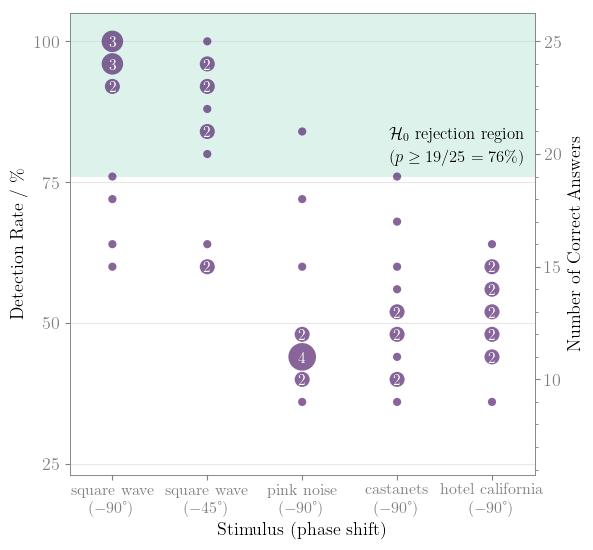
\includegraphics[width=0.67\textwidth]{graphics/scatter}
\end{figure}
\end{frame}
%
%
%
\section{Conclusion}
\begin{frame}{Conclusion}
constant phase shifter is known as fractional Hilbert transform

audibility depends on audio material and amount of constant phase shift

\begin{columns}[c]
\column{0.45\textwidth}
\begin{figure}
\includegraphics[width=1\textwidth]{graphics/spectra_filterorder510}
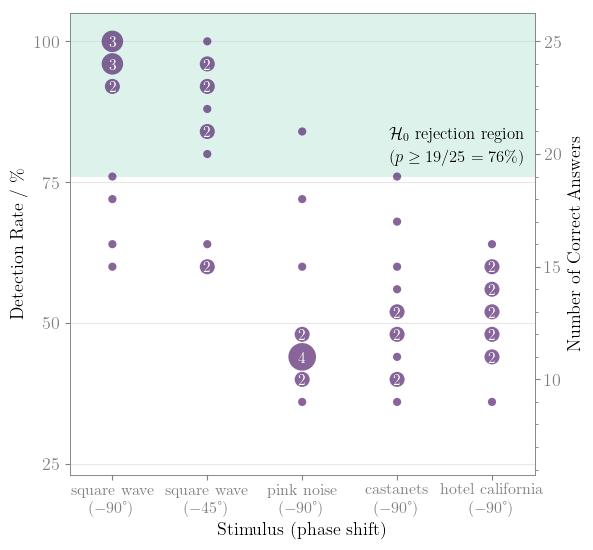
\includegraphics[width=1\textwidth]{graphics/scatter}
\end{figure}
\column{0.45\textwidth}
\only<1>{
\begin{itemize}
\item very sensitive to square wave bursts
\item likely sensitive for transient signals and lowpass filtered noise
\item audibility for musical content not yet shown
\item training improves sensitivity...
\end{itemize}
}
\only<2>{

\textcolor{colnonzero}{\textbf{Outlook}}

trained experts achieve

%\textcolor{colnonzero}{pink noise}: 40 correct detections $(p<2.1 \cdot 10^{-10})$
%\textcolor{colnonzero}{castanets}: 28 correct $(p<0.022)$ and 39 correct $(p<2.9\cdot10^{-9})$

\textcolor{colnonzero}{pink noise}: 95\% correct answers $(p<2.1 \cdot 10^{-10})$

\textcolor{colnonzero}{castanets}: 92\% correct answers $(p<2.9\cdot10^{-9})$
\vspace*{0.5cm}

\tiny ABX test design with assumed effect size $g =	0.25$,
$\alpha = 0.05$, power $1-\beta=0.95 \rightarrow
\frac{\geq 27\,\text{correct trials}}{42\,\text{total trials}}$
}

\end{columns}
\end{frame}
%
%
%
\maketitle
%
%
%
\section{Appendix}
%
%
%
\begin{frame}[noframenumbering]{Periodic Convolution}
Impulse response for $\varphi=-\frac{\pi}{4}$
\begin{figure}
\includegraphics[width=0.75\textwidth]{graphics/periodic-ir}
\end{figure}
\end{frame}
%
%
%
\begin{frame}[noframenumbering]{Quantization Filter Coefficients}
\begin{figure}
\includegraphics[width=\textwidth]{graphics/amplitude-decay}
\end{figure}
\end{frame}
%
%
%
\begin{frame}[noframenumbering]{Crest Factor}
\begin{figure}
\includegraphics[width=\textwidth]{graphics/crest-factor-and-square-waves}
\end{figure}
\end{frame}
%
%
%
\begin{frame}[noframenumbering]{Crest Factor}
\begin{figure}
\includegraphics[width=\textwidth]{graphics/crest-factor}
\end{figure}
\end{frame}
%
%
%
\end{document}
